\documentclass[12pt,a4paper]{report}
\usepackage[utf8]{inputenc}
\usepackage{amsmath}
\usepackage{amsfonts}
\usepackage{amssymb}
\usepackage{hyperref}
\usepackage{graphicx}
\usepackage[numbers]{natbib}
\usepackage{hyperref}
\usepackage{float}
\def\UrlBreaks{\do\/\do-}
\graphicspath{ {images/} }
\usepackage[a4paper,top=3cm,bottom=2cm,left=3cm,right=3cm,marginparwidth=1.75cm]{geometry}

\begin{document}
\sloppy
\begin{titlepage}
	\centering
	
\includegraphics[width=0.15\textwidth]{Brighton-University-logo.png}\par
	{\scshape\LARGE University of Brighton\par}
	\vspace{1cm}
	{\scshape\Large Interim planning and Investigation report\par}
	\vspace{1.5cm}
	{\huge\bfseries Generation of Raspbian images\par}
	\vspace{2cm}
	{\Large\itshape Adam Pietrzycki\par}14843569
	\vfill
	supervised by\par
	Dr.~Aidan \textsc{Delaney}
	\vfill
	{\large \today\par}
\end{titlepage}

\begin{abstract}
As of the 8th September 2016, in a blog post by raspberry pi founder Eben Upton \citep{blog}, mentions that the ten millionth raspberry pi has just been sold. The official operating system for these devices is called Raspbian, it is a port of Debian which is available as a standalone image or in a 'New Out Of the Box Software' package for beginners. 'NOOBS' is pre-installed on SD cards that can be bought from many retailers, before the images can be burned to the cards they need to be somehow generated. The current method of generating these images can be found on GitHub \citep{pi-gen}, it is a set of shell scripts which from the commits look to be predominantly maintained by a single developer. The problem with this is that if the developer decided to move on and depart from the project it might take some time before someone else understands the code well enough to be able to carry it on; this can be simply described as the 'Bus Factor.' \citep{bus} Since the release of the raspberry pi in February 2012, new tools have been developed and standards decided; so it might be a nice idea to freshen up the current method.      
\end{abstract}

\pagebreak
\tableofcontents
\pagebreak

\chapter{Introduction}
\section{Aims}
The overall aim of the project is to show that the current code base, which generates the Raspbian images can be re-written and re-designed to make use of open source tools and a 'human friendly data serialization standard,' \citep{yaml} called YAML. 
\section{Objectives}
The objectives can be separated into two different categories; project and personal. These will provide an idea of the project structure and will help towards a successful completion. 
\subsection{Project}
\begin{itemize}
\item{Write code that utilizes open source tools and language standards.}
\item{Generate Raspbian images at a faster speed.}
\item{Give options to users for easy image customization.}
\item{Get feedback from the Raspberry Pi foundation.}
\end{itemize}  
\subsection{Personal}
\begin{itemize}
\item{Learn shell scripting.}
\item{Learn a provision management tool.}
\item{Understand Linux on a more complex level.}
\item{Expand knowledge of virtualization.}
\end{itemize}  

\chapter{Background Research}
\section{Deployment Management Tools}
There are many deployment management tools to choose from, all offer different benefits and are backed by various companies. A comparison of tools has been covered in detail at Openstack's Summit \citep{openstack} of which are referenced throughout the deployment management sections below.    	
\subsection{Puppet}
Puppet \citep{puppet} released 2005, is one of the earliest approaches to configuration management. It uses a mixture of Ruby and a custom language for writing manifests and templates. The puppet master provides commands to its agents over XML-RPC, it works over HTTP(S) and requires an agent to be installed on the host. Puppet makes use of a WebUI and has reporting tools built in but at the the same time has been described as having a steep learning curve for new users, requiring the user to learn a new language is not ideal; this rules out the use of Puppet for this project. 
\subsection{Chef}
Chef \citep{chef} released 2008, takes many things from Puppet. They both use Ruby for writing templates and configuration, Chef seems to take on the idea that you should automate everything. The clients poll the Chef server by default every 30 minutes to pull the latest instructions, which are carried out over SSH. Chef still requires an agent to be installed on the server. Overall Chef seems to be most suitable for enterprise solutions due to the vast amount of features available, though it requires extensive understanding to set up and use. It is too feature packed for this kind of project.
\subsection{Salt}
Salt \citep{salt} released 2012, is quite different compared to the previous two. It is written in Python and instructions are done over SSH, this is to allow for parallel execution whilst keeping it highly scalable. You can have a centralized salt master control other masters who then control minions, essentially anything can control everything. The difference now is that there is an optional GUI available. This could of been a suitable tool for the project but the documentation can be challenging to understand.
\subsection{Ansible}
Ansible \citep{ansible} released 2013, is really similar to Salt. It is written in Python and uses SSH to push instructions to the servers, the only prerequisite server side is that python has to be installed; there is no need for any agents. There is no need for any central server and it is very easy to get started. A big factor that makes Ansible very suitable for this project is that the configuration is done in YAML, it is a standard that anyone can get their head around in no time at all. Having looked greatly at Ansible it is possible to use a chroot as a host, this can be integrated perfectly with parts of the current Raspbian generation code base.     
\section{Virtualization}
When deploying code it is normally recommended to test on the same operating system as the current server to reduce the possibility of errors. There are many ways you can set up virtual systems in order to test on a local system or a local network.  
\subsection{ESXi}
ESXi \citep{esxi} is a bare-metal hypervisor by VMWare, it is installed directly on hardware which allows you to install virtual machines on top of it. This form of virtualization of normal within enterprise as it is more cost efficient than running multiple separate physical servers. VMWare do offer products which are designed to be ran on client devices rather than servers but most of them are paid products and there are free alternatives available.
\subsection{VirtualBox}
VirtualBox \citep{virtualbox} is an open source solution by Oracle, it is supported on a large platform of systems and it is free to use for personal and enterprise reasons. Due to the nature of the licensing people have developed alternative front-ends and extended functionality in various scenarios. 

\subsection{Docker}
Docker \citep{docker} is a really interesting approach to virtualization, instead of creating multiple virtual machines on a hypervisor, Docker can run multiple individual containers using one machine. This removes the need for having multiple guest operating systems making it lightweight and really scalable.  
\subsection{Vagrant}
Vagrant \citep{vagrant} is built by HashiCorp, it is one of those tools that works on top of VirtualBox. Vagrant is a really simply way to set up a complete development environment in a productive manner. This is now becoming the most popular virtualization tool for developers as it works cross platform. 
\subsection{QEMU}
QEMU \citep{qemu} is also open source, it achieves near native performance but most \\importantly it can virtualize different CPU architectures. This is used in the current method Raspbian images are generated. 

\section{Current generation method}
\subsection{Analysis}
The current method of generating Raspbian images makes use of QEMU-user, chroot and a set of shell scripts. To get it working you have to run the scripts as root on a Debian machine, make sure that the dependencies are installed or the build will fail. If running on a virtualized Debian machine you have to make sure the virtual disk it large enough, if you are using Vagrant then Debian bento boxes \citep{bento} work best. Overall the general structure of the code base is set up rather neatly but once you start looking at the actual code it can take some time to get your head around it. Stages are separated out and contain their own set of specific folders and scripts within them, though there is a scripts folder in the root directory that seems to be called at the very start.  
\subsection{Potential improvements}
Having looked over the current code base and spoken to the original author a few things can be looked at to improve the overall performance.
\begin{itemize}
  \item{Don't copy each stage, use qcow and branch each stage instead}
  \item{Run zipping/tarring in parallel, look at lzop}
  \item{Export stages can be run at the same time as the next build stage}
\end{itemize}


\chapter{Project Planning}
\section{Standards and quality checks}
Ansible uses the YAML notation, which alone is a standard that can be used across multiple languages. There is in depth Ansible documentation \citep{ansibledoc} which provides you with examples of code and references on what the best code practise is, this ensures the quality of code is as best as possible.
\section{Methodologies}
There are many methodologies \citep{methodologies} available when it comes to project management. Different types of projects have their preferred project methodology.
\subsection{Waterfall}
Waterfall is a 'traditional, sequential methodology,' which has proven to work for projects over the years. The only problem with it is that it does not adapt well to software development as software is very likely to change; changes are disruptive to the overall project.  
\subsection{Agile}
Agile is the preferred methodology when dealing with software development, the reason for it is that it allows for iterative cycles without affecting the overall progress of the project. Agile allows for testing to be integrated from the very beginning, this is essential for the success of the project.  

\section{Stakeholders}
There are many stakeholders with various interests connected to this project, some direct and others indirect. 

\begin{itemize}
  \item{Stakeholder - Dr. Aidan Delaney}
    \subitem{Interest - Project supervisor}
    \subitem{Communication - Meetings in person, Email}
  \item{Stakeholder - Raspberry Pi Foundation}
    \subitem{Interest - New method of generating Raspbian images}
    \subitem{Communication - Email, IRC, GitHub}
  \item{Stakeholder - Developers}
    \subitem{Interest - Able to easily customise Raspbian image}
    \subitem{Communication - Email, IRC, GitHub}  
  \item{Stakeholder - Raspberry Pi users}
    \subitem{Interest - Unknowingly using images generated using this project}
    \subitem{Communication - None}
\end{itemize}

\section{Project schedule}
An Gantt chart can be used to estimate the length of the project. This is helpful as it can be used to determine if a project will be complete on time. 
\begin{figure}[h]
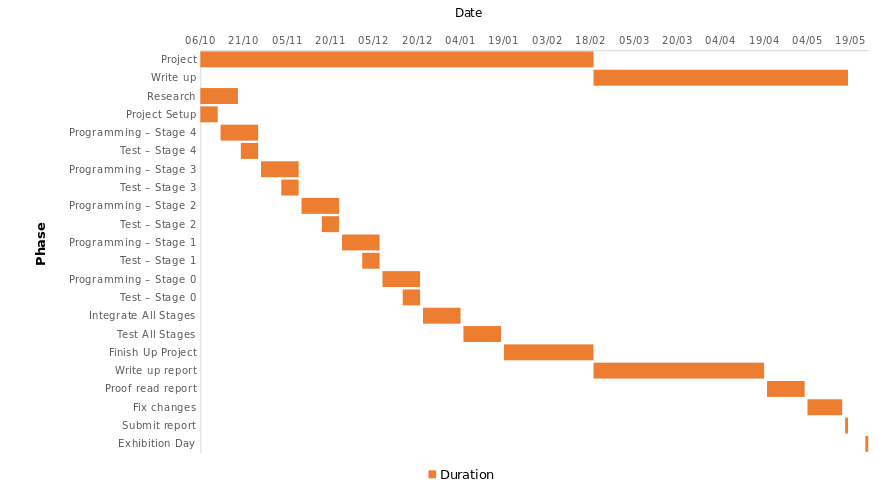
\includegraphics[width=15cm]{schedule}
\caption{Project estimation Gantt chart}
\centering
\end{figure}

\subsection{Risks}
There are a few things that could risk this project, though you can not prevent everything.
\begin{itemize}
  \item{A programming stage takes longer than expected.}
    \subitem{This could potentially delay the project.}
  \item{Ansible does not support a native function.}
    \subitem{Code would have to be rewritten, might take longer than expected.}
  \item{GitHub could be down.}
    \subitem{People would not be able to clone the project.}
  \item{Current method of generation might break things if updated.}
    \subitem{Latest code would have to be integrated during the project.}
\end{itemize}

\addcontentsline{toc}{chapter}{Bibliography}
\bibliographystyle{plainnat}

\begin{thebibliography}{9}
\bibitem{blog}
Raspberry Pi. (2016). Ten millionth Raspberry Pi, and a new kit.
\\\url{https://www.raspberrypi.org/blog/ten-millionth-raspberry-pi-new-kit/}
\\\textit{This is the official Raspberry Pi Foundation blog ran by the founder Even Upton, there are a few interesting statistics on this blog.}

\bibitem{pi-gen}
Raspberry Pi. (2016). RPi-Distro/pi-gen.
\\\url{https://github.com/RPi-Distro/pi-gen}
\\\textit{The original code base for generating Raspbian images can be found here, the project pi-gen can be found here \url{https://github.com/adampie/pi-gen}.}

\bibitem{bus}
Wikipedia. (2016). Bus Factor.
\\\url{https://en.wikipedia.org/wiki/Bus_factor}
\\\textit{A Wikipedia page describing the 'Bus Factor'.}

\bibitem{yaml}
YAML. (2009). \%YAML 1.2.
\\\url{http://yaml.org/}
\\\textit{Main website for YAML, contains links to projects using various languages integrating YAML.}

\bibitem{openstack}
Openstack. (2015). Chef vs. Puppet vs. Ansible vs. Salt - What's Best for Deploying and Managing OpenStack?.
\\\url{https://www.openstack.org/summit/tokyo-2015/videos/presentation/chef-vs-puppet-vs-ansible-vs-salt-whats-best-for-deploying-and-managing-openstack}
\\\textit{Video and slides for the Openstack Summit, information in the deployment management tools section was referenced from this talk. Really good and in depth comparison}

\bibitem{puppet}
Puppet. (2016). Puppet - The shortest path to better software.
\\\url{https://puppet.com/}
\\\textit{Official site for Puppet}

\bibitem{chef}
Chef. (2016). Chef – Automate Your Infrastructure.
\\\url{https://www.chef.io/chef/}
\\\textit{Official site for Chef}

\bibitem{salt}
Glauser, R. (2016). SaltStack automation for CloudOps, ITOps \& DevOps at scale.
\\\url{https://saltstack.com/}
\\\textit{Official site for Salt}

\bibitem{ansible}
Red Hat. (2016). Ansible is Simple IT Automation.
\\\url{https://www.ansible.com/}
\\\textit{Official site for Ansible}

\bibitem{esxi}
VMWare. (2016). vSphere ESXi Bare-Metal Hypervisor.
\\\url{http://www.vmware.com/products/esxi-and-esx.html}
\\\textit{Official site for ESXi}

\bibitem{virtualbox}
Oracle. (2016). Oracle VM VirtualBox.
\\\url{https://www.virtualbox.org/}
\\\textit{Official site for VirtualBox}

\bibitem{docker}
Docker. (2016). Docker.
\\\url{https://www.docker.com/}
\\\textit{Official site for Docker}

\bibitem{vagrant}
HashiCorp. (2016). Vagrant by HashiCorp.
\\\url{https://www.vagrantup.com/}
\\\textit{Official site for Vagrant}

\bibitem{qemu}
QEMU. (2016). QEMU - Open source processor emulator.
\\\url{http://wiki.qemu.org/Main_Page}
\\\textit{Official site for QEMU}

\bibitem{bento}
Chef. (2016). Bento by Chef.
\\\url{http://chef.github.io/bento/}
\\\textit{A list of Vagrant images that have a large virtual disk suitable for using with this project.}

\bibitem{ansibledoc}
Ansible. (2016). Ansible Documentation.
\\\url{http://docs.ansible.com/}
\\\textit{Official Ansible documentation, includes code examples useful for project.}

\bibitem{methodologies}
Wrike. (2016). Project Management Guide for Beginners.
\\\url{https://www.wrike.com/project-management-guide/methodologies/}
\\\textit{Explanation of choosing project management methodologies, helped get a quick overall idea.}

\end{thebibliography}
\end{document}


